\documentclass[
  lang=cn,
  degree=master,
  zhuanshuo,
  openany,oneside
  % openright,blankleft,twoside
]{nuaathesis}

\graphicspath{{./fig/},{./logo/},{../logo/}}

\iffalse
  % 本块代码被上方的 iffalse 注释掉,如需使用,请改为 iftrue
  % 使用 Noto 字体替换中文宋体、黑体
  \setCJKfamilyfont{\CJKrmdefault}[BoldFont=Noto Serif CJK SC Bold]{Noto Serif CJK SC}
  \renewcommand\songti{\CJKfamily{\CJKrmdefault}}
  \setCJKfamilyfont{\CJKsfdefault}[BoldFont=Noto Sans CJK SC Bold]{Noto Sans CJK SC Medium}
  \renewcommand\heiti{\CJKfamily{\CJKsfdefault}}
\fi

\iffalse
  % 本块代码被上方的 iffalse 注释掉,如需使用,请改为 iftrue
  % 在 XeLaTeX + ctexbook 环境下使用 Noto 日文字体
  \setCJKfamilyfont{mc}[BoldFont=Noto Serif CJK JP Bold]{Noto Serif CJK JP}
  \newcommand\mcfamily{\CJKfamily{mc}}
  \setCJKfamilyfont{gt}[BoldFont=Noto Sans CJK JP Bold]{Noto Sans CJK JP}
  \newcommand\gtfamily{\CJKfamily{gt}}
\fi


% 设置基本文档信息,\linebreak 前面不要有空格,否则在无需换行的场合,中文之间的空格无法消除
\nuaaset{
  title = {踝关节外骨骼的控制系统设计},
  author = {陈建宇},
  college = {自动化学院},
  advisers = {张娟娟 副教授,吕品 副教授},
  % applydate = {二〇一八年六月}  % 默认当前日期
  %
  % 本科
  major = {自动化},
  studentid = {051510626},
  classid = {0315106},
  % 硕/博士
  majorsubject = {\LaTeX},
  researchfield = {\LaTeX 排版},
  libraryclassid = {TP371},       % 中图分类号
  subjectclassid = {080605},      % 学科分类号
  thesisid = {1028704 18-S000},   % 论文编号
}
\nuaasetEn{
  title = {Design of Control System for Ankle Exoskeletons},
  author = {JianYuChen},
  college = {NUAA},
  majorsubject = {Automation},
  advisers = {Prof.~JuanJuanZhang},
  degreefull = {Master of Engineering},
  % applydate = {June, 8012}
}

% 摘要
\begin{abstract}
  外骨骼是一种用来提高人体机能的可穿戴设备,在军事作战、医疗康复等领域具有重要意义。提高人机交互的舒适性与安全性,为当前外骨骼领域的研究热点。本文研究对象为一种踝关节式外骨骼,在现有机械结构的基础上,对外骨骼传感系统、力矩控制方法、人在环中优化进行了研究。

  可靠、准确、稳定的人机交互数据对外骨骼而言至关重要。本文首先搭建了外骨骼的传感系统。针对所研究的踝关节式外骨骼,使用应变片测量外骨骼对人体施加的力矩,通过足底开关和惯性测量单元分析人体步态运动信息,通过EMG信号测量肌肉的激活水平。

  在传感系统的基础上,本文对外骨骼的力矩控制方法进行了研究。力矩控制由上层控制器与底层控制器组成,上层控制器用来产生期望力矩曲线,底层控制器实现对期望力矩曲线的跟踪。对于上层控制器,本文采用基于时间的直接力矩控制,并通过三次函数插值得到期望力矩曲线。针对底层控制器,本文提出了三种控制算法,设计了四种不同组合的控制器,通过实验发现融合三种控制算法的控制器具有较好的力矩跟踪效果。

  最后,本文研究了人在环中的参数优化方法。针对最佳助力模式因人而异的问题,本文以穿戴者的肌肉激活水平为目标函数,使用贝叶斯优化外搜寻最佳助力参数。实验表明,外骨骼系统能够在五分钟内寻找到最佳助力参数。在最佳助力参数下,受试者肌肉激活度平均下降12.2\%。

\end{abstract}
\keywords{外骨骼, 力矩控制, 人在环中优化}

\begin{abstractEn}
  Exoskeletons are wearable device used to enhance human mobility,which are significant in military, medical rehabilitation and many other fields.Improving the comfort and safety during human-machine interaction has become a hotspot in exoskeleton research.The research object of this paper is an ankle type exoskeleton.Based on the existing mechanical structure of an ankle exoskeleton,we study the sensing system,torque control method and human-in-loop optimization.

  Accurate and reliable sensor information is critical for exoskeleton.In this paper,we first develop a sensing system.The torque exerted on exoskeleton was measured by strain gauge,human gait information was analyzed by plantar switch,and muscle activation level was measured by EMG signal.

  Based on the sensing system,we study torque control method,which consists of upper controller and lower controller.The upper controller is used to generate desired torque curve,and the lower controller is used for tracking the desired torque curve.This paper adopts the direct torque control based on time,and obtains the desired torque curve by cubic spline interpolation.We proposes three control algorithms and design four different combinations of lower controller.Through experiments,we found that the controller contains all three algorithms has better torque tracking performance.

  Finally,we study human-in-loop optimization.We find that optimal assistance mode varies from person to person,which can be searched by optimization method.In the paper,the target function is human muscle activation level,and Bayesian Optimization was chosen to search optimal assistance.During five experiments,the exoskeleton system successfully searched the optimal assistance mode in five minutes.Under optimal assistance parameters,the muscle activation level of human subject decreased by 12.2\% on average.
\end{abstractEn}
\keywordsEn{exoskeleton, torque control, human in loop optimization}

% 请按自己的论文排版需求,随意修改以下全局设置

\usepackage{subfig}
\usepackage{rotating}
\usepackage[usenames,dvipsnames]{xcolor}
\usepackage{tikz}
\usepackage{pgfplots}
\pgfplotsset{compat=1.16}
\pgfplotsset{
  table/search path={./fig/},
}
\usepackage{ifthen}
\usepackage{longtable}
\usepackage{siunitx}
\usepackage{listings}
\usepackage{multirow}
\usepackage[bottom]{footmisc}
\usepackage{pifont}

\lstdefinestyle{lstStyleBase}{%
  basicstyle=\small\ttfamily,
  aboveskip=\medskipamount,
  belowskip=\medskipamount,
  lineskip=0pt,
  boxpos=c,
  showlines=false,
  extendedchars=true,
  upquote=true,
  tabsize=2,
  showtabs=false,
  showspaces=false,
  showstringspaces=false,
  numbers=left,
  numberstyle=\footnotesize,
  linewidth=\linewidth,
  xleftmargin=\parindent,
  xrightmargin=0pt,
  resetmargins=false,
  breaklines=true,
  breakatwhitespace=false,
  breakindent=0pt,
  breakautoindent=true,
  columns=flexible,
  keepspaces=true,
  framesep=3pt,
  rulesep=2pt,
  framerule=1pt,
  backgroundcolor=\color{gray!5},
  stringstyle=\color{green!40!black!100},
  keywordstyle=\bfseries\color{blue!50!black},
  commentstyle=\slshape\color{black!60}}

%\usetikzlibrary{external}
%\tikzexternalize % activate!

\newcommand\cs[1]{\texttt{\textbackslash#1}}
\newcommand\pkg[1]{\texttt{#1}\textsuperscript{PKG}}
\newcommand\env[1]{\texttt{#1}}

\theoremstyle{nuaaplain}
\nuaatheoremchapu{definition}{定义}
\nuaatheoremchapu{assumption}{假设}
\nuaatheoremchap{exercise}{练习}
\nuaatheoremchap{nonsense}{胡诌}
\nuaatheoremg[句]{lines}{句子}

% \includeonly{content/start,}

\begin{document}

\makecover
\makedeclare
\frontmatter
\makeabstract
% 如果需要调整目录层级数量的话,取消下一行注释,数字含义: 0=chapter, 1=section, 2=subsection
% \setcounter{tocdepth}{1}
\nuaatableofcontents
\nuaalistoffigurestables
% sorry, but the guy is too lazy to make an English notation demo.

\chapter*{Notations}

\noindent\begin{tabu} to \textwidth {|X[l]|p{4.5cm}|X[l]|p{4.5cm}|}\hline
$A, A_0$ & 状态方程矩阵 & $e$ & 误差绝对值 \\ \hline
$a$ & 重心到前轴的距离 & $e_i$ & 误差变化率 \\ \hline
$a_0, a_1, a_2, a_3$ & 多项式系数 & $F(\omega)$ & 多项式 \\ \hline
$a_{c0}$ & 加速度变量 & $F_i, \theta _i$ & Fadeev递归算法中间变量 \\ \hline

\multirow{2}{*}{$a_{s1}, a_{s0}$} & \multirow{2}{4.5cm}{连轴器及传动轴简化模型传递系数} &
$F_X$ & 汽车总制动力 \\ \cline{3-4}
& & $F_Y$ & 汽车总侧向力 \\ \hline

$a_y$ & 横向加速度 & $f_b$ & 轮胎制动力 \\ \hline
$a_{yc}$ & 横向加速度极限值 & $f_{bi}, f_{ci}$ & 各轮制动力和侧偏力 \\ \hline
$\tilde{a}_0, \tilde{a}_1, \tilde{a}_2, \tilde{a}_3$ & 多项式系数 & $G$ & 状态方程矩阵 \\ \hline
$B, B_0, B_1$ & 状态方程矩阵 & $g$ & 重力加速度 \\ \hline
$B_{w1}, B_{w2}$ & 状态方程矩阵 & $H$ & 汽车重心高度 \\ \hline
$b$ & 重心到后轴的距离 & $H(j \omega)$ & 频响函数 \\ \hline
$b_0, b_1, b_2, b_3$ & 多项式系数 & $h$ & 汽车重心到侧倾中心的距离 \\ \hline
$b_m$ &电机阻尼比系数 & $h_r$ & 汽车侧倾中心高度 \\ \hline
\end{tabu}

\chapter*{Abbreviations}

\noindent\begin{tabu} to \textwidth {|X[1,c]|X[4,c]|}\hline
Abbreviation & Full Form \\ \hline
WSN & Wireless Sensor Networks \\ \hline
CAM & Center Angle Method \\ \hline
LEACH & Low-Energy Adaptive Clustering Hierarchy \\ \hline
\end{tabu}


\mainmatter

\chapter{はじめに}

日本語専修じゃないので、中国語で書きたいっと思います。

\zhcn{除了中文、英文外,\nuaathesis{} 也支持日语论文,论文主体为日语,其中偶尔出现小段汉语。

由于目标用户的母语是汉语,所以请读者参阅用汉语写的文档 nuaathesis.pdf。
中文的示例文档中大部分内容是通用的,里面包含一些常用宏包的使用方法。
本文档只介绍一些日语 \LaTeX{} 的使用注意事项。}


\section{\zhcn{\LaTeX{} 环境准备}}

\zhcn{请参照文档、中英文示例论文中介绍的方法,该方法也会一同安装日语 \LaTeX{} 所需要的工具、宏包。}

\section{\zhcn{编译论文}}

\zhcn{这一步与其他语言的论文有很大不同,由于使用了 \CTeX{} 来提供中文支持,
因此只能使用 up\LaTeX{} 引擎来编译。编译前需要确认论文目录下存在以下文件:}
\begin{itemize}
  \item \zhcn{nuaathesis.cls、nuaathesis.bst 等文件(与其他语言相同)}
  \item \zhcn{ctex-engine-uptex.def(请参阅 pdf 文档,里面描述了如何获取、修改该文件)}
  \item \zhcn{.latexmkrc(如果打算使用 latexmk 来编译的话)}
\end{itemize}

\zhcn{编译文档时推荐使用 latexmk,假定论文的名字叫做 master.tex,具体执行的命令如下:}
\begin{shell}
latexmk -pdfdvi master
\end{shell}

\zhcn{实质上,它执行了以下几条命令:}
\begin{shell}
uplatex master
upbibtex master
uplatex master
uplatex master
dvipdfmx master
\end{shell}

\chapter{特色功能}

本章节介绍由 \nuaathesis{} 提供的特有的宏。

\section{定理环境}

\nuaathesis{} 没有定义任何定理环境,
但提供了三个宏 \cs{nuaatheorem(g|chap|chapu)} 来定义不同编号方法的定理环境。
\begin{enumerate}
  \item \cs{nuaatheoremg} 的编号只有一个数字;
  \item \cs{nuaatheoremchap} 的编号由“章节.序号”构成,不同的定理环境的编号是独立的,
  它们的数字编号会重复,如“\autoref{ex:oneplus}”后面可能出现“\autoref{non:dora}”;
  \item \cs{nuaatheoremchapu} 的编号也是由“章节.序号”构成,
  但它们的数字编号是统一的,同一个数字不会重复出现(仅限用\cs{nuaatheoremchapu}声明的定理环境之间)。
  如“\autoref{def:distance}”后面\textbf{不会}出现“假设~2.1”,但可能出现“定义~2.2”或“\autoref{assume:fail}”;
\end{enumerate}

由于学校没有规定计数的编号,所以所有的定理环境应该由作者来决定编号方式,
这也意味着所有的定理环境都要由作者来定义(这不是 \nuaathesis{} 在偷懒哦)。

顺便一提,在同一章里同时出现两种编号方式的定理环境,很可能造成混乱,
所以请合理安排定理环境的编号方式。以下开始举栗子。

\subsection*{样例}

\begin{definition}[欧几里得距离]
\label{def:distance}
点$\mathbf{p}$与点$\mathbf{q}$的\textbf{欧几里得距离},是连接该两点的线段($\overline{\mathbf{pq}}$)的长度。

在笛卡尔坐标系下,如果 $n$维欧几里得空间下的两个点 $\mathbf{p}=(p_1, p_2, \dots, p_n)$ 与点
$\mathbf{q} = (q_1, q_2, q_3, \dots, q_n)$,那么点$\mathbf{p}$与点$\mathbf{q}$的距离,
或者点$\mathbf{q}$与点$\mathbf{p}$的距离,由以下公式定义:
\begin{align}
\label{equ:1}
d(\mathbf{p},\mathbf{q}) = d(\mathbf{q},\mathbf{p}) & = \sqrt{(q_1-p_1)^2 + (q_2-p_2)^2 + \cdots + (q_n-p_n)^2} \\
\label{equ:2}
& = \sqrt{\sum_{i=1}^n (q_i-p_i)^2}
\end{align}
\end{definition}

\begin{proof}
由\cs{nuaatheorem(g|chap|chapu)}定义的定理环境支持 \cs{autoref},
比如在\autoref{def:distance}中,\autoref{equ:2}是\autoref{equ:1}的简写。

但是 \cs{autoref} 只能在 \cs{ref} 加上前缀,无法加上后缀。
所以上一句话的后半部分,更推荐手工来写标注 “(\ref{equ:2}) 是 (\ref{equ:1}) 的简写”。

定理环境里面可以换行,不过证明与其他定理环境稍有不同,它是单独定义实现的,
因此末尾会有一个(帅气的) QED 符号。
\end{proof}

\begin{assumption}
\label{assume:fail}
假设本身就不成立
\end{assumption}

\begin{lines}
\label{s1}
例句1
\end{lines}

\section{参考文献}
\label{sec:bib}
参考文献应该以上标的形式标注于论述之后,就像这样:

\begin{itemize}
\item 研究表明\cite{r1},早睡早起有益身体健康。
\item 如果想同时引用多个文献\cite{r2,r3,r4,r6},只需要在 \verb|cite{}| 中用逗号分开\texttt{citeKey}就好。
\end{itemize}

本模板保留了 \cquthesis{} 里的 \texttt{inlinecite},但请注意它不符合学校的要求,无论本科还是硕士、博士,
请\textbf{谨慎}使用:
文献\inlinecite{r6}表明,文献\inlinecite{r7,r8,r9}所述的情况是有理论依据的。

\nuaathesis 格式测试,学校的参考文献格式并不是 GB7714-2015,所以追加一些测试样例。
《要求》里列出的格式有:
\begin{enumerate}
  \item 连续出版物\cite{n11,n12}:[序号]作者.文题.刊名,年,卷号(期号):起~止页码.
  \item 专译集\cite{n21,n22}:[序号]作者.书名(译者).出版地:出版者,出版年:起~止页码.
  \item 论文集\cite{n31,n32}:[序号]作者.文题.编者,文集名,出版地:出版者,出版年:起~止页码.
  \item 学位论文\cite{n41,n42,n43}:[序号]姓名.文题,[XX学位论文].授予单位所在地:授予单位,授予年.
  \item 专利\cite{n51,n52,n53}:[序号]申请者.专利名,国名,专利文献种类,专利号,出版日期.
  \item 技术标准\cite{n61,n62,n63}:[序号]发布单位,技术标准代号,技术标准名称,出版地:出版者,出版日期.
\end{enumerate}

注:目前实现的格式仍然与《要求》有点差异:
\begin{enumerate}
  \item 《要求》里论文集的编者、文集名、出版地是逗号分隔,而目前是点号分隔;
  \item 《要求》的学位论文用中文注明学位,目前没实现;
  \item 在信息缺失的情况下,《要求》貌似直接把对应字段省略,目前仍显示“XX不详”。
\end{enumerate}

\chapter{定理环境·下}

本章演示使用 \cs{nuaatheoremchap} 定义的定理环境,注意它们的数字编号是可以重复的。

\section{演示一级标题}
\subsection{演示二级标题}
\subsubsection{演示三级标题}

\begin{nonsense}
\label{non:dora}
哆啦A梦写的论文被拒稿的可能性很高
\footnote{出处:\url{https://www.math.kyoto-u.ac.jp/~arai/latex/presen2.pdf} 的最后一页}。
\end{nonsense}

\begin{exercise}
\label{ex:oneplus}
证明$1+1 = 2$。
\footnote{Testing footnote with English spaces}
\end{exercise}

\begin{nonsense}[右边的胡诌是真的]
“练习”与“胡诌”定理环境的编号是相互独立的,它们的数字编号允许重复,
如“\autoref{non:dora}”和“\autoref{ex:oneplus}”。
\end{nonsense}

\begin{exercise}
按照本文所演示的方法,利用 \cs{nuaatheorem(g|chap|chapu)} 来定义您的论文中所需要的定理环境。
\end{exercise}

\begin{lines}
\label{s2}
例句2
\end{lines}

\autoref{s2} 没有章节编号,它是全局编号的,它可以用在外国语学院论文中来枚举例句。

\chapter{使用示例}

本章介绍一些常用的宏包的常用方法,希望能为读者写作时提供参考。

\section{插图}

首先讨论一下插图的格式,在 \LaTeX{} 环境下,
\begin{enumerate}
\item 推荐使用宏包来绘制插图,如 \pkg{tikz},它兼容所有 \LaTeX{} 环境,
字体能与全文统一,质量最佳,但是需要的学习成本较大。
请务必先阅读 \pkg{tikz} 文档的第1章教程,
然后可以去 texample\footnote{\url{http://texample.net/tikz}} 等网站上找类似的例子,
也可以使用 GeoGebra\footnote{\url{https://www.geogebra.org}} 之类的工具来生成\TeX 代码,
效果可以参见\autoref{fig:tikzrot};
\item 其次推荐使用其他绘图工具生成的 \verb|PDF|、 \verb|EPS| 格式的矢量图,
\verb|svg| 格式可以通过 inkscape 软件转换成带 \TeX{}文本代码的 \verb|PDF|。效果可以参见\autoref{fig:logo};
\item 当然,\verb|PNG|、 \verb|jpeg| 之类的位图格式也能做插图;
\item 最后,不要忘记论文是\textbf{单色印刷}的,请确保插图在黑白打印的情况下的清晰度。
\end{enumerate}

\begin{figure}[htb]
  \newcounter{density}
  \setcounter{density}{20}
  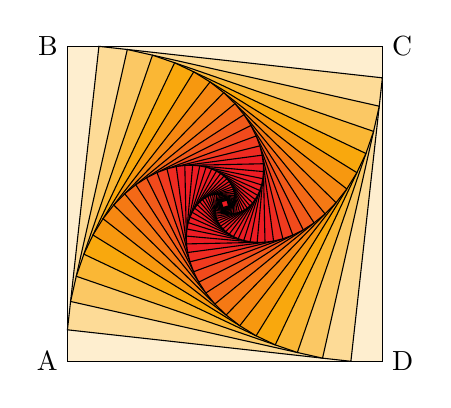
\begin{tikzpicture}
  \newcounter{density}
  \setcounter{density}{20}
  \def\couleur{Dandelion}
  \path[coordinate] (0,0) coordinate(A)
              ++( 90:4cm) coordinate(B)
              ++(0:4cm) coordinate(C)
              ++(-90:4cm) coordinate(D);
  \draw (A) node[left] {A}
    (B) node[left] {B}
    (C) node[right] {C}
    (D) node[right] {D};
  \draw[fill=\couleur!\thedensity] (A)--(B)--(C)--(D)--cycle;
  \foreach \x in {1,...,40}{%
      \pgfmathsetcounter{density}{\thedensity+25}
      \setcounter{density}{\thedensity}
      \path[coordinate] coordinate(X) at (A){};
      \path[coordinate] (A) -- (B) coordinate[pos=.1](A)
                          -- (C) coordinate[pos=.1](B)
                          -- (D) coordinate[pos=.1](C)
                          -- (X) coordinate[pos=.1](D);
      \draw[fill=\couleur!\thedensity] (A)--(B)--(C)--(D)--cycle;
  }
\end{tikzpicture}

  \caption{tikz例子}
  \label{fig:tikzrot}
\end{figure}

\begin{figure}[htb]
  
\includegraphics[width=4cm]{nuaa-logo.pdf}
  \caption{一个校徽}
  \label{fig:logo}
\end{figure}

如果需要多个插图共用一个题注的话,需要加载额外的宏包,
一般选用 \pkg{subcaption} 或 \pkg{subfig},这两个宏包是互斥的。
需要注意的是 \pkg{subcaption} 貌似与 \pkg{geometry} 有些冲突,
会导致多行的图表的最后一行无法居中,而 \pkg{geometry} 是设置页边距的必用宏包。
所以个人推荐使用  \pkg{subfig},效果可以参考\autoref{fig:sub2}。

\begin{figure}[htb]
  \subfloat[左边的大校徽\label{fig:sub1}]{
\includegraphics[width=4cm]{nuaa-logo.pdf}}\quad
  \subfloat[短标题:小校徽][小校徽,题注很长,不过请各位放心,它会自动换行\label{fig:sub2}]
  {
\includegraphics[width=3cm]{nuaa-logo.pdf}}
  \caption{包含两张图片的插图}
  \label{fig:subfigs}
\end{figure}

如果需要插入图表的话,可以考虑使用 \pkg{pgfplots} 宏包,效果参见\autoref{fig:plots};
也可以用 Matplotlib、MatLab、Mathematica 之类的工具导出成兼容格式的图片。

\begin{figure}[htb]
  \subfloat[二维图像\label{fig:func}]{%\documentclass{ctexart}
%\usepackage{pgfplots}
%\pgfplotsset{compat=1.16}
%\begin{document}
\begin{tikzpicture}
  \pgfplotstableread[
    % col sep=comma
  ]{data/plot_2d.csv}{\Data}
  \begin{axis}[
    width=.45\textwidth,
    xmin=0, xmax=16, xtick distance=4,
    xlabel={序列},
    ymin=0, ymax=1,
    ylabel={正确率},
    grid=both,
    legend pos=south east,
  ]
    \addplot+ table[x=idx, y=parray] {\Data};
    \addlegendentry{环境1};
    \addplot+[mark=o] table[x=idx, y=pround] {\Data};
    \addlegendentry{环境2};
  \end{axis}
\end{tikzpicture}
%\end{document}
} \quad
  \subfloat[三维图像\label{fig:sum}]{%\documentclass{minimal}
%\usepackage{pgfplots}
%\pgfplotsset{compat=1.16}
%\begin{document}
\begin{tikzpicture}
  \pgfplotstableread[
    % col sep=comma
  ]{data/plot_3d.csv}{\Data}
  \begin{axis}[
    width=.45\textwidth,
    view={-30}{30},
    xmin=0, xmax=16, xtick distance=4,
    xlabel={Num},
    ymin=1, ymax=20, ytick distance=5,
    ylabel={Round},
    zmin=0, zmax=1, ztick distance=.2,
    zlabel={PDF},
    z tick label style={
      /pgf/number format/.cd,
        fixed,
        fixed zerofill,
        precision=1,
      /tikz/.cd
      },
    grid=major,
  ]
    \addplot3[
      surf,
      mesh/rows=17,
      patch type=rectangle,
      opacity=1,fill opacity=0.1,
      colormap/cool
    ] table[x=num, y=round, z=p] {\Data};
  \end{axis}
\end{tikzpicture}
%\end{document}
}
  \caption{拙作中利用 \pkg{pgfplot} 绘制的图表}
  \label{fig:plots}
\end{figure}

如果真的需要让十几张图片共用一个题注的话,
需要手工拆分成多个 \env{float} 并用 \cs{ContinuedFloat} 来拼接,
不过直接多次使用 \cs{caption} 会在图表清单里产生多个重复条目,需要一点点小技巧
(设置图表目录标题为空)。
建议将浮动位置指定为 \verb|t|,以确保分散至多页的图能占用整个页面,手工分页才能靠谱。
效果可以参见\autoref{fig:subfigss} 的\autoref{fig:logo6}。

\begin{figure}[t]
  \subfloat[校徽$\times 1$]{
\includegraphics[width=4cm]{nuaa-logo.pdf}}\quad
  \subfloat[校徽$\times 2$]{
\includegraphics[width=.4\textwidth]{nuaa-logo.pdf}}\\
  \subfloat[校徽$\times 3$]{
\includegraphics[width=.4\textwidth]{nuaa-logo.pdf}}\quad
  \subfloat[校徽$\times 4$]{
\includegraphics[width=4cm]{nuaa-logo.pdf}}
  \caption{包含多张图片的插图}
  \label{fig:subfigss}
\end{figure}
\begin{figure}[t]
  \ContinuedFloat
  \subfloat[校徽$\times 5$]{
\includegraphics[width=4cm]{nuaa-logo.pdf}}\quad
  \subfloat[校徽$\times 6$ \label{fig:logo6}]{
\includegraphics[width=4cm]{nuaa-logo.pdf}}\\
  \subfloat[校徽$\times 7$]{
\includegraphics[width=4cm]{nuaa-logo.pdf}}\quad
  \subfloat[校徽$\times 8$]{
\includegraphics[width=4cm]{nuaa-logo.pdf}}
  % 指定图表清单中的标题为[],即可将其消除,避免目录中出现重复条目
  \caption[]{包含多张图片的插图(续)}
\end{figure}

如果需要插入一张很大的图片的话,可以使用 \pkg{rotating} 提供的 \env{sidewaysfigure},
它能将插图放置在单独的页面上,如果文档使用 \verb|twoside| 选项的话,它会根据页面方向,
设置 \ang{90} 或 \ang{270} 旋转,可能需要编译两遍才能设置正确的旋转方向。
不过可能有一个问题,\env{sidewaysfigure} 中使用 \cs{subfloat} 可能无法准确标号,
需要手工重置 \texttt{subfigure} 计数器。
效果参见\autoref{fig:fullpage1} 和\autoref{fig:fullpage2}。

\setcounter{subfigure}{0}
\begin{sidewaysfigure}
  \subfloat[First caption\label{fig:fp1}]{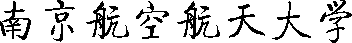
\includegraphics[width=.8\textheight]{nuaa-jianqi.pdf}} \\
  \subfloat[Second caption]{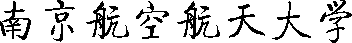
\includegraphics[height=2cm]{nuaa-jianqi.pdf}}
  \caption{一幅占用完整页面的图片}
  \label{fig:fullpage1}
\end{sidewaysfigure}

\setcounter{subfigure}{0}
\begin{sidewaysfigure}
  \subfloat[First caption]{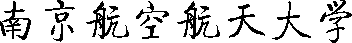
\includegraphics[height=2cm]{nuaa-jianqi.pdf}} \\
  \subfloat[Second caption]{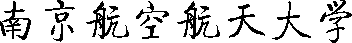
\includegraphics[width=.8\textheight]{nuaa-jianqi.pdf}}
  \caption{又一幅占用完整页面的图片}
  \label{fig:fullpage2}
\end{sidewaysfigure}

\section{表格}

由于封面页,本模板预先加载了 \pkg{array} 和 \pkg{tabu},如果需要其他表格的宏包,
请自行加载。

如果需要插入一个简易的表格,可以只使用 \env{tabular} 环境,如\autoref{tab:city}。
\begin{table}[htb]
  \caption[城市人口]{城市人口数量排名 (source: Wikipedia)\label{tab:city}}
  \begin{tabular}{lr}
    \toprule
    城市 & 人口 \\
    \midrule
    Mexico City & 20,116,842\\
    Shanghai & 19,210,000\\
    Peking & 15,796,450\\
    Istanbul & 14,160,467\\
    \bottomrule
  \end{tabular}
\end{table}

也可以使用 \env{tabu} 环境,它可以更灵活地设置列宽,但它有一些 bug,如\autoref{tab:tabu}。
\begin{table}[htb]
  \caption{\env{tabu} 注意事项 \label{tab:tabu}}
  \begin{tabu} to .9\textwidth {XX[2]<{\strut}} \toprule
    默认列 & 有修正的列 \\ \midrule
    \env{tabu} 的 bug? \par This line is BAD & 注意左侧最后一行后的垂直空格 \\ \midrule
    注意对比最后一行 &
      bug 会影响多行的 \env{tabu} 表格 \par
      bug 的修正方法是在段落后面加 \cs{strut} \par
      This line is Good \\ \midrule
    垂直居中没效果 & 改用 \env{tabular} \\ \midrule
    与新版 \pkg{array} 不兼容 & 谨慎使用,切勿用 \texttt{tabu spread} \\ \bottomrule
  \end{tabu}
\end{table}

如果需要对某一列的小数点对齐,或者带有单位,或者需要做四舍五入的处理,可以尝试配合 \pkg{siunitx} 一起使用。
非常推荐看一下 \pkg{siunitx} 文档的,至少看一下“Hints for using siunitx”一节的输出结果,
\autoref{tab:xmpl:mixed} 来自于该文档的 7.14 节。

\begin{table}[htb]
  \caption{Tables where numbers have different units}
  \label{tab:xmpl:mixed}
  \begin{tabular}
    {
      >{$}l<{$}
      S[table-format = 2.3(1)]
      S[table-format = 3.3(1)]
    }
    \toprule
      & {One} & {Two} \\
    \midrule
    a / \si{\angstrom}   &  1.234(2) &   5.678(4) \\
    \beta / \si{\degree} & 90.34(4)  & 104.45(5)  \\
    \mu / \si{\per\mm}   &  0.532    &   0.894    \\
    \bottomrule
  \end{tabular}
  \hfil
  \begin{tabular}
    {S[table-format=1.3]@{\,}s[table-unit-alignment = left]}
    \toprule
    \multicolumn{2}{c}{Heading} \\
    \midrule
    1.234 & \metre   \\
    0.835 & \candela \\
    4.23  & \joule\per\mole \\
    \bottomrule
  \end{tabular}
\end{table}

如果表格内容很多,导致无法放在一页内的话,需要用 \env{longtable} 或 \env{longtabu} 进行分页。
\autoref{tab:performance} 是来自 \cquthesis{} 的一个长表格的例子。

\begin{longtable}[c]{c*{6}{r}}
	\caption[实验数据]{实验数据,这个题注十分的长,注意这在索引中的处理方式,还有 \cs{caption} 后面的双反斜杠}\label{tab:performance}\\
	\toprule
	\multirow{2}{*}{测试程序} & \multicolumn{1}{c}{正常运行} & \multicolumn{1}{c}{同步} & \multicolumn{1}{c}{检查点} & \multicolumn{1}{c}{卷回恢复}
	& \multicolumn{1}{c}{进程迁移} & \multicolumn{1}{c}{检查点} \\
	& \multicolumn{1}{c}{时间 (s)}& \multicolumn{1}{c}{时间 (s)}&
	\multicolumn{1}{c}{时间 (s)}& \multicolumn{1}{c}{时间 (s)}& \multicolumn{1}{c}{时间 (s)}& \multicolumn{1}{c}{文件 (KB)} \\ \midrule
	\endfirsthead
	\multicolumn{7}{c}{\nuaafontcaption 续表~\thetable\hskip1em 实验数据}\\
	\toprule
	\multirow{2}{*}{测试程序} & \multicolumn{1}{c}{正常运行} & \multicolumn{1}{c}{同步} & \multicolumn{1}{c}{检查点} & \multicolumn{1}{c}{卷回恢复}
	& \multicolumn{1}{c}{进程迁移} & \multicolumn{1}{c}{检查点} \\
	& \multicolumn{1}{c}{时间 (s)}& \multicolumn{1}{c}{时间 (s)}&
	\multicolumn{1}{c}{时间 (s)}& \multicolumn{1}{c}{时间 (s)}& \multicolumn{1}{c}{时间 (s)}& \multicolumn{1}{c}{文件(KB)} \\ \midrule
	\endhead
	\hline
	\multicolumn{7}{r}{续下页}
	\endfoot
	\endlastfoot
	CG.A.2 & 23.05 & 0.002 & 0.116 & 0.035 & 0.589 & 32491 \\
	CG.A.4 & 15.06 & 0.003 & 0.067 & 0.021 & 0.351 & 18211 \\
	CG.A.8 & 13.38 & 0.004 & 0.072 & 0.023 & 0.210 & 9890 \\
	CG.B.2 & 867.45 & 0.002 & 0.864 & 0.232 & 3.256 & 228562 \\
	CG.B.4 & 501.61 & 0.003 & 0.438 & 0.136 & 2.075 & 123862 \\
	CG.B.8 & 384.65 & 0.004 & 0.457 & 0.108 & 1.235 & 63777 \\
	MG.A.2 & 112.27 & 0.002 & 0.846 & 0.237 & 3.930 & 236473 \\
	MG.A.4 & 59.84 & 0.003 & 0.442 & 0.128 & 2.070 & 123875 \\
	MG.A.8 & 31.38 & 0.003 & 0.476 & 0.114 & 1.041 & 60627 \\
	MG.B.2 & 526.28 & 0.002 & 0.821 & 0.238 & 4.176 & 236635 \\
	MG.B.4 & 280.11 & 0.003 & 0.432 & 0.130 & 1.706 & 123793 \\
	MG.B.8 & 148.29 & 0.003 & 0.442 & 0.116 & 0.893 & 60600 \\
	LU.A.2 & 2116.54 & 0.002 & 0.110 & 0.030 & 0.532 & 28754 \\
	LU.A.4 & 1102.50 & 0.002 & 0.069 & 0.017 & 0.255 & 14915 \\
	LU.A.8 & 574.47 & 0.003 & 0.067 & 0.016 & 0.192 & 8655 \\
	LU.B.2 & 9712.87 & 0.002 & 0.357 & 0.104 & 1.734 & 101975 \\
	LU.B.4 & 4757.80 & 0.003 & 0.190 & 0.056 & 0.808 & 53522 \\
	LU.B.8 & 2444.05 & 0.004 & 0.222 & 0.057 & 0.548 & 30134 \\
	CG.B.2 & 867.45 & 0.002 & 0.864 & 0.232 & 3.256 & 228562 \\
	CG.B.4 & 501.61 & 0.003 & 0.438 & 0.136 & 2.075 & 123862 \\
	CG.B.8 & 384.65 & 0.004 & 0.457 & 0.108 & 1.235 & 63777 \\
	MG.A.2 & 112.27 & 0.002 & 0.846 & 0.237 & 3.930 & 236473 \\
	MG.A.4 & 59.84 & 0.003 & 0.442 & 0.128 & 2.070 & 123875 \\
	MG.A.8 & 31.38 & 0.003 & 0.476 & 0.114 & 1.041 & 60627 \\
	MG.B.2 & 526.28 & 0.002 & 0.821 & 0.238 & 4.176 & 236635 \\
	MG.B.4 & 280.11 & 0.003 & 0.432 & 0.130 & 1.706 & 123793 \\
	MG.B.8 & 148.29 & 0.003 & 0.442 & 0.116 & 0.893 & 60600 \\
	LU.A.2 & 2116.54 & 0.002 & 0.110 & 0.030 & 0.532 & 28754 \\
	LU.A.4 & 1102.50 & 0.002 & 0.069 & 0.017 & 0.255 & 14915 \\
	LU.A.8 & 574.47 & 0.003 & 0.067 & 0.016 & 0.192 & 8655 \\
	LU.B.2 & 9712.87 & 0.002 & 0.357 & 0.104 & 1.734 & 101975 \\
	LU.B.4 & 4757.80 & 0.003 & 0.190 & 0.056 & 0.808 & 53522 \\
	LU.B.8 & 2444.05 & 0.004 & 0.222 & 0.057 & 0.548 & 30134 \\
	EP.A.2 & 123.81 & 0.002 & 0.010 & 0.003 & 0.074 & 1834 \\
	EP.A.4 & 61.92 & 0.003 & 0.011 & 0.004 & 0.073 & 1743 \\
	EP.A.8 & 31.06 & 0.004 & 0.017 & 0.005 & 0.073 & 1661 \\
	EP.B.2 & 495.49 & 0.001 & 0.009 & 0.003 & 0.196 & 2011 \\
	EP.B.4 & 247.69 & 0.002 & 0.012 & 0.004 & 0.122 & 1663 \\
	EP.B.8 & 126.74 & 0.003 & 0.017 & 0.005 & 0.083 & 1656 \\
	\bottomrule
\end{longtable}

\section{数字与国际单位}

本模板预加载 \pkg{siunitx} 来格式化文中的内联数字,该宏包有大量可定制的参数,
请务必阅读其文档,并在文档导言部分设置格式。

\begin{itemize}
  \item 旋转角度为 \ang{90}、\ang{270}
  \item 分辨率 \num{1920x1080} 的像素数量约为 \num{2.07e6}
  \item 电脑显示器的像素间距为 \SI{1.8}{\nm}、\SI{180}{\um} 还是 \SI{18}{\mm}?
  \item 重力加速度 $g=\SI{9.8}{\kg\per\square\second}$、
  $g=\SI[inter-unit-product=\ensuremath{{}\cdot{}}]{9.8}{\kg\per\square\second}$,
  亦或 $g=\SI[per-mode=symbol]{9.8}{\kg\per\square\second}$
\end{itemize}

\section{中英文之间空格}

很遗憾,目前 \LaTeX{} 和 \CTeX{} 虽然能处理普通汉字与英文之间的间隔,
但是汉字与宏之间的空格仍然需要手工调整,请务必按以下的规则撰写原稿:
\begin{itemize}
  \item[\ding{51}] 如\autoref{fig:sub2} 所示:\verb|如\autoref{fig:sub2} 所示|,这个宏返回的是“图 x.xx”,
  所以前面两个汉字之间不能加空格,后面数字与汉字之间必须加空格;
  \item[\ding{51}] 距离为 1.7~个天文单位:\verb|距离为 1.7~个天文单位|,前面可以不加空格(\CTeX 会修正),
  后面必须加 \verb|~| 以防止在 “1.7”与“个”之间换行。此时更推荐写成 \SI{1.7}{au}:\verb|\SI{1.7}{au}|。
\end{itemize}


\appendix
% 如果需要附录的话,在这里 include
\chapter{后记}

\section{v0.9a后记——Old Jack 的吐槽}

\verb!\begin{轻松+愉快}!

Old Jack 他有点累......

Old Jack 两年前就开始关注南航毕设的\LaTeX 模板了,但是两年了还没有任何有实际意义的新动作,所以Old Jack 就亲自操刀制作了新的一版。虽然很多代码都是从其他模板中直接摘抄过来的,但是这也是\TeX 最普遍、最快捷的学习\&开发方法。一开始 Old Jack 也想造轮子,但是轮子真的不好造。

在制作过程中遇到了几个关键性的问题:
\begin{itemize}
  \item 前文提到的三种粗体
  \item nuaa.png源文件和页眉制作
  \item 英文字母、章节标题莫名其妙的加粗
  \item 脚注相对页脚线的位置
\end{itemize}

第一个问题 Old Jack 曾经用\TeX 中伪粗体(FakeBold)的方法实现过,但是效果并不好,而且当时受到最后一个问题的强烈影响,不得不使用其他字体来解决这个问题。

第二个问题 Old Jack 开始是使用官方模板中的图片,但是分辨率太低,效果很差。于是 Old Jack Google以图搜图找到了现在的这个文件的源文件,经过了一系列不可描述的操作后得到了现在的 nuaa.png 。页眉的制作也让 Old Jack 很头疼,论文要求论文到顶端和底端的距离分别为2.5cm和2.0cm,Old Jack 很naive的就给geometry设置了这个数值,但是效果和官方模板差了很多,于是 Old Jack 只好一点一点地调试,达到了近似官方模板的效果。页脚和官方模板有细微的区别,Old Jack 认为这无伤大雅,是要罗马数字和阿拉伯数字编号正确应该就可以了。

第三个问题是一个非常奇怪的问题。使用伪粗体时所有标题全都加粗了,非常难看,经过了代码重构和不停地调试解决了这个问题。在模板完成99\% 后发现最后致谢中的英文字体全都加粗了, Old Jack 几次审视代码和调试都没有解决。偶然间,Old Jack 将全部主要文件全部提取出来,放入另一个文件夹,然后重新编译就解决了这个问题!当然后来发现代码中确实有一个地方有小问题\textbf{可能}会影响,但是这不是上一次出错的原因。Old Jack 对于各位使用模板的南航学子以及其他可能会参考此模板的\TeX 爱好者提了一个建议:\textbf{任何语言,任何代码出现莫名其妙的问题时,换一个文件夹,改一下名字,重新跑一下,可能会得到意想不到的结果。}当然这不是万能的解决方法。

第四个问题就如第一章中脚注和页脚线的情况,感觉两条线很别扭。 Old Jack 犹豫了很久,最后没有采用将脚注放在页脚线下的方案,因为 Old Jack 觉得还是两条线的方案好看。对于想要将脚注放在页脚线下方的同学,可以在主文件中取消注释那段代码,来实现所需要的效果。

Old Jack 他完成了模板的再制作,但是他没有心气再写出一篇能够指导大家使用\LaTeX 的文档了(好吧,Old Jack 他承认懒是一部分因素),望大家谅解 Old Jack。

\verb!\end{轻松+愉快}!

\section{v1.0后记}

Old Jack 非常高兴,因为他不是一个人在战斗。再次感谢张一白、王成欣、曾宪文、Gavin Lee等人的工作,没有他们,\nuaathesis 不会像现在这么美丽。

经过\nuaathesis~Group的努力和测试,\nuaathesis 迎来了v1.0版,也就是第一个正式发行版。一路走来也是有些坎坷,各种各样的小问题一直困扰着我们,其实v1.0 也还有着一些细小的问题尚未解决。不过Old Jack请大家放心,这些小问题不影响模板的使用。很多已经被我们解决的小问题比如页眉的大小位置,中英文字体是否正确,摘要的章节标题不能是加粗的宋体等等,老师可能不去管这些,甚至注意不到有什么区别。相比之下,重要的地方是:公式、图表的编号,图表和文本的位置,参考文献的格式等等才是老师关注的点。很多地方只是我们几个人为了追求和office模板尽可能接近,才不断地进行修改调整,也是有点讽刺。

写毕设论文的时候,Old Jack 不止一次看到隔壁室友调公式内容,Mathtype和Office装了卸,卸了装、调公式编号、调标题位置和大小、调首行缩进、调段间距等等等等,看着他们搞得焦头烂额的,Old Jack 都觉得心累。打印时也是这样,有太多的人在打印店不停地修改自己的论文,有因为office和wps不兼容修改的,有office版本不兼容修改的,有因为页眉页脚错误修改的等等。然而 Old Jack 他在写论文时从来没有担心过这些事情(当然,作为模板开发者 Old Jack 确实操心了很多,2333),他也第一次真正体会到了什么叫做专注于内容,真的挺轻松的(表格是例外)。

对于模板的推广,Old Jack觉得使用人数仍然不会太多,毕竟\LaTeX 的群众基础太小,除了8院,其他学院对公式的需求整体来讲并不迫切,Old Jack 猜测大部分知道、了解\LaTeX 的同学是通过数学建模竞赛这个途径才学习了\LaTeX ;同时因为涉及到学习新的程序语言,时间成本也较大,所以很多同学的学习意愿不高。不过\nuaathesis 的目标人群本来也不是全校所有学生,Old Jack 的思路,Old Jack 相信也是\nuaathesis~Group其他开发者的思路是:
\begin{enumerate}
  \item 为自己服务,这是\nuaathesis~Group开发模板的第一动力;
  \item 对已经掌握\LaTeX 基本语法的同学,\nuaathesis~Group为他们在毕业设计时能更轻松地撰写论文,提供平台和机会;
  \item 对准备学习\LaTeX 以及已经学习了一点\LaTeX 的同学,\nuaathesis~Group为他们提供学下去的动力和平台。
\end{enumerate}

即将毕业了,回首大学四年, Old Jack 做过疯狂的事情,也找到了一份看起来还可以的工作,只觉得还没对学校做过什么有用的事情,尽管 Old Jack 对学校其实并不是很有感情。完成了这个模板后,至少 Old Jack 可以减少一个遗憾,然后离开学校了。虽然这不是什么惊天动地的工作,但是至少 Old Jack 做了件他认为还算有意义的事情。Old Jack应该还会再维护\nuaathesis 一段时间,期待有后继者能够接过火炬,继续完善并推广\nuaathesis 。

想说的可能也就这么多了,Old Jack out!

\hfill 0813~王志浩,2017.6.24

\section{v2.0 后记 by yzwduck}

也是两年前开始关注南航毕设的\LaTeX 模板了,但直到毕业前,都没能去静下心来学习\LaTeX。

现在差不多本科毕业一年,或者说,一年后要开写硕士学位论文了,
本打算照着 CQUThesis 来造轮子的时候,逛纸飞机\footnote{论坛还活着吗?该不会已经沦落为老人的回忆了吧。 ——2018.10.10}
看到 \nuaathesis~v1.0 发布了。
非常激动、也很自愧,同样是经历了大学四年的人,我没能把这模板做出来。

于是马上把两年前为了模板而画的校名(矢量图)传了上去\footnote{\url{https://github.com/nuaatug/nuaathesis/commit/24fa82e}}。

原本打算在 v1.0 版的基础上修改的,但因为行间距设置有问题,封面与 Word 模板也有点差异,
还要再加入硕/博士的模板,于是干脆改成 \texttt{Documented LaTeX Source (.dtx)},
方便以后写模板的文档。

做模板过程中遇到的大问题,在于如何正确理解学校对论文格式的要求。
虽然有《本科毕业设计(论文)撰写格式要求》、《研究生学位论文撰写要求》,
但这些要求依然不够细致,因为那些要求都是假定你用 Word 来写论文的,要求里的内容是 Word 设置的操作方法,
所以还要先学习 Word 的排版算法。虽然这不是热门的资料,而且还有 CJK 独有的坑,
幸好有人把 Word 排版算法解释得非常详细,这个模板才能避免大量使用测量得到的魔数。
但还有很多细节部分,因为能力有限,没能实现。

最后容我吐槽一下学校的 Word 模板,我觉得那个 Word 模板可能从最初做出来后,就基本没有变化。
那个“最初”或许可以追溯到上个世纪。很多编号的事情都要由手工来完成,比如说目录页码、
各级标题的编号、题注等。这些完全可以自动编号的工作,如果要手工做的话【掀桌颜文字】。

\section{v2.1 后记 by yzwduck}

转眼间一年过去,又到了写毕业论文的时候了。

翻了一下代码的 commit 记录(部分非公开),这一年间只有加起来两、三个星期在做这个论文模板,
已经无法用“懒”这字来描述鄙人的状态了。

不过也有几件值得小小炫耀一下的事,终于把中/英/日多国语的坑填了不少,至少能编译出对应语言的论文来;
为了减少重复代码,使用一些宏包造了 \CTeX{} 的几个轮子,从而实现一个 class 文件能支持三国语言。

为了检验模板的效果,鄙人从知网上找了两篇论文,试着用 \nuaathesis{} 模板排版了一下(节选),又发现了不少问题。
因此目前 \nuaathesis{} 应该还有相当多的问题的,但没有用户的话,由于鄙人能力有限,难以发现,
还请各位使用 \nuaathesis{} 的先行者们(Pioneers) 能反馈意见和建议。

愿所有使用 \nuaathesis{} 的人,不会被评审老师指责格式问题。


\backmatter
% 如果参考文献使用 biber
\bibliographystyle{nuaabib}   % 参考文献的样式
\bibliography{bib/sample}   % 参考文献,即 bib/sample.bib 文件(纯文本)
% 如果打算手写参考文献
\chapter{\bibname}

\begin{manref}
\item \label{ref:hint} 本节演示如何手写参考文献目录
\item 如果论文能用 biber 来管理参考文献的话,请使用 biber,不要手写
\item 如果实在不方便用 biber 的话,可以使用这种方法来手写参考文献。格式完全手写会有点繁琐,而且不能在正文中引用。比如:
\item \label{ref:man} KANAMORI H. Shaking without quaking[J]. Science, 1998, 279(5359): 2063.
\item 吴云芳.面向中文信息处理的现代汉语并列结构研究[D].北京:北京大学,2003[2013-10-14].
\end{manref}

示例:[\ref{ref:hint}] 这种写法不符合学校的要求,推荐使用这种写法\mcite{ref:man}。


\chapter{Acknowledge}

Thanks for reading, and have a nice day.

\chapter{\zhcn{在学期间的研究成果及学术论文情况}}

\subsection*{\zhcn{攻读硕士学位期间发表(录用)论文情况}}

\begin{enumerate}
  \item Lamport, Leslie. LATEX: a document preparation system: user's guide and reference manual. Addison-wesley, 1994.
\end{enumerate}

\subsection*{\zhcn{研究生期间参与的科研项目}}

\begin{enumerate}
  \item \zhcn{国家自然科学基金} (No.12345678)
\end{enumerate}


\end{document}
